\chapter{Metodologia de Pesquisa}
A metodologia de pesquisa utilizada nesse trabalho, possui aspectos qualitativos que permitem identificar a importância deste trabalho junto à comunidade de especialistas da área de saúde e também possui aspectos quantitativos que demonstram que a abordagem utilizada consegue diferenciar indivíduos com portadores da doença de parkinson perante indivíduos que não desenvolveram a doença por intermédio de sensores de movimento e de força. O desfecho da pesquisa se fará com o resultado tanto da pesquisa qualitativa quanto da pesquisa quantitativa.

\section{Desenho da Pesquisa} \label{sec:desenho_pesquisa}
Para uma melhor compreensão da pesquisa temos o Desenho da Pesquisa a ser realizada na Figura \ref{figure:desenho_pesquisa} e a descrição de cada um dos passos.


A Problemática desse trabalho, já foi descrita na Seção \ref{section:problematica}. A revisão da literatura irá consistir de uma descrição sobre a doença estudada como estudo de caso (Doença de Parkinson) que está descrito no Capítulo \ref{section:doenca_parkinson}, bem como da possibilidade de integrar o monitoramento da doença de Parkinson por intermédio de jogos eletrônicos. 


\begin{figure}[!htbp]
    \centering
    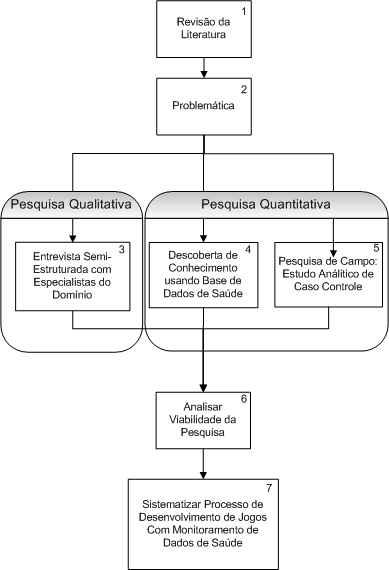
\includegraphics[width=.7\textwidth]{./img/metodologia-pesquisa.png}
    \caption{Desenho da Pesquisa}
    \label{figure:desenho_pesquisa}
\end{figure}

\section{Pesquisa Qualitativa}
Essa pesquisa tem como objetivo identificar a importância de realizar o monitoramento de dados de saúde por intermédio jogos eletrônicos. Em um primeiro momento, serão verificados junto a comunidade médica a relevância desse trabalho e se este poderia auxiliar no monitoramento dos sintomas parkinsonianos. 

Os pesquisadores que adotam a abordagem da pesquisa qualitativa a fazem por sua flexibilidade, sem regras rígidas, aplicáveis a uma ampla gama de casos e formalizações pré-definidas, possibilitando a construção de modelos abrangentes \cite{Gom00}. 
Nesse estudo a pesquisa qualitativa está orientada a um estudo de caso, partindo da análise das expressões e comportamento das pessoas. Na busca por entender os fenômenos sociais complexos, o estudo de caso permite uma investigação significativa nas mudanças desses processos\cite{Yin05}.

Por se tratar de um estudo empírico, utilizamos a pesquisa qualitativa por envolver uma grande variedade de técnicas para levantamento de informações (entrevistas, observações, histórico, interações, artefatos e ferramentas utilizadas) \cite{FLI04}.

%Partindo da problemática da pesquisa \ref{section:problematica}, essa pesquisa busca identificar por intermédio de uma técnica de pesquisa qualitativa de Entrevista Semi-Estruturada junto a profissionais de saúde a importância do monitoramento dos dados de saúde

%esse texto abaixo está repetido na problemática



%Nessa seção iremos descrever a metodologia de pesquisa adotada no
%estudo. Na seção 1 apresenta-se o desenho da pesquisa com suas
%respectivas etapas. Na seção 2 apresenta os aspectos metodológicos
%do estudo. Na seção 3 apresenta-se a operacionalização das
%variáveis. Por último, na seção 4, é apresentada a base metodológica
%do estudo.
\subsection{Entrevista Semi-Estruturada Com Especialistas do Domínio (3)}\label{section:entrevista_semi-estruturada}

O objetivo deste procedimento foi entender como é feito o acompanhamento dos sintomas da doença de parkinson juntamente aos profissionais de saúde (neurologistas que prescrevem a dosagem medicamentosa e fisioterapeutas que fazem o acompanhamento motor do paciente ao longo de seu tratamento). Os mesmos foram indagados se poderia haver melhora na tomada de decisão caso eles pudessem acompanhar o surgimento dos sintomas em diferentes momentos do dia por intermédio de um monitoramento frequente dos sintomas. Procurou-se encontrar dentro do contexto de estudo, a importância do monitoramento de dados de saúde e os benefícios trazidos por este.

\subsubsection{Perfil dos participantes}

O público alvo da pesquisa são profissionais de saúde especialistas em doenças neurológicas e acompanhamento motor que realizam acompanhamento de pacientes com a doença de parkinson. Devido a sua formação, esses profissionais são aptos a fornecer subsídios para o desenvolvimento da solução proposta neste trabalho.

Logo no início da entrevistas devem ser obtidas informações sobre a formação acadêmica, tempo de experiência e área de atuação.

%, de modo auxiliar na visualização do contexto da pesquisa uma tabela foi elaborada com o perfil de cada participante. %COLOCAR REFERENCIA DE TABELA%


As entrevistas foram realizadas de maneira presencial, onde primeiramente fez-se perguntas não estruturadas e havendo uma maior estruturação no decorrer da entrevista com a preocupação de que seja evitada a referência do entrevistador seja sobre os pontos de vista do entrevistado conforme prega o método científico \cite{FLI04}. Durante a pesquisa foi utilizado recursos de gravação, de modo a facilitar a transcrição dos dados coletados. %[Uma tabela resumindo as principais características das pessoas]

\subsubsection{Entrevista com Profissionais de Saúde Especialistas em Neurologia} 
Essa etapa da pesquisa foi baseada num conjunto de questões/guia vide Apêndice \ref{apendice:entrevista-semi-estruturada}, onde nem todas as perguntas elaboradas foram utilizadas.

Para a construção do questionário foi realizada uma análise sobre a doença de parkinson e sintomas que pudessem ser monitorados usando sensores, para a construção do questionário foram utilizadas diretrizes médicas da Doença de Parkinson ~\cite{protpar010,national2006parkinson} e da tabela UPDRS ~\cite{updrs87} usada para avaliação do progresso da doença ~\cite{updrs87}.

A entrevista semi-estruturada realizada teve um total de 15 perguntas agrupadas em 3 seções, com os seguintes temas: sintomas da doença de parkinson, monitoramento da saúde motora e os benefícios advindos do monitoramento. Devido as diferenças existentes na abordagem utilizada por cada profissional o entrevistador poderá selecionar as questões de acordo com suas características.

%\section{Analisar Viabilidade da Pesquisa (6)} A análise de resultados servirá de base para o desenvolvimento do processo proposto. Dando o suporte necessário para a seleção de um conjunto de ferramentas a serem incorporadas na execução do processo. 
%A análise do resultado está descrita no \chapref{chapter:analise_resultados}.

\subsection{Análise da Entrevista Semi-Estruturada}

Como o método de pesquisa da entrevista Semi-Estruturada é qualitativo. Será realizada uma pesquisa qualitativa assistida por computador utilizando-se o \textit{software} QDA Miner \cite{qda13}. Este \textit{software} permite a análise qualitativa das informações obtidas em modo texto. Software dessa natureza auxiliam o pesquisador na organização dos registros da pesquisa e das interpretações dos mesmos. A escolha dessa ferramenta é justificada pela dificuldade de classificar e analisar os dados obtidos. Nessa análise somente foram levadas em consideração as atividades referentes ao acompanhamento dos sintomas motores em pacientes de parkinson e como um possível cenário que permitisse o monitoramento desses sintomas por intermédio de jogos eletrônicos poderia auxiliar os pacientes e também os profissionais de saúde.

\subsubsection{Instrumento de Análise dos Dados da Pesquisa Qualitativa} \label{section:analise_dados} 

A interpretação de dados é o cerne da pesquisa qualitativa. Tem como função desenvolver a teoria, servindo ao mesmo tempo de base para a decisão sobre quais dados adicionais devem ser coletados \cite{FLI04}.

É importante que seja realizada a codificação seletiva, para que seja elaborada a categorização essencial sobre todas as categorias envolvidas \cite{FLI04}. O pesquisador precisa decidir quais os fenômenos salientes e ponderá-los de forma a ter como resultado uma categoria central juntamente com as categorias a ela relacionadas.

O procedimento da interpretação dos dados, assim como a integração de material adicional, é encerrado quando atinge a "saturação teórica", quando o avanço da codificação não atinge mais novos conhecimentos \cite{FLI04}.

Para análise dos textos provenientes da pesquisa (transcrição da entrevista com os Neurologistas e Fisioterapeutas especialistas em Neurologia) foi utilizada a codificação seletiva através de criação de categorias a \emph{posteriori}. As categorias foram criadas e organizadas de acordo com o conteúdo de cada texto. As respostas de cada participante foram analisadas e a partir da identificação das categorias, incluídas na árvore de categorias do QDA Miner \cite{qda13}, que possui a transcrição de cada questionário e interação ocorrida. Admitindo-se que uma classificação, para ser adequada não pode ser feita arbitrariamente, a categorização da árvore será criada e reformulada várias vezes, durante o processo de análise de acordo com \cite{FLI04}.

Por fim, com base na análise do texto, foram verificados dificuldades, necessidade, importância e viabilidade da pesquisa do ponto de vista dos profissionais de saúde.
 
\section{Descoberta de Conhecimento usando Base de Dados de Saúde}
Para esse estudo, foram utilizados dados do \textit{PhysioBank} ~\cite{physionet}. O \textit{PhysioBank} armazena sinais fisiológicos e dados relacionados a comunidade de pesquisa biomédica, incluindo sinais vitais, motores de indivíduos saudáveis e de pacientes com uma variedade de sintomas como distúrbios neurológicos ou envelhecimento. 

\subsection{Materiais}
Para a presente pesquisa, foi utilizada a base de dados "\textit{Parkinson´s Disease Database}" ~\cite{physionet} a qual contém as medidas da marcha de 93 pacientes com doença de Parkinson idiopática (idade média: 66,3 anos, 63$\%$ homens) e 73 controles saudáveis ​​(com idade média de 66,3 anos, 55$\%$ homens). Esse banco de dados inclui os registros da \ac{fvrs} de indivíduos enquanto eles caminhavam normalmente em seu próprio ritmo por aproximadamente 2 minutos em um terreno plano. Debaixo de cada pé foram postos oito sensores (Figura \ref{fig:posicaosensores}) (\texit{Ultraflex Computer Dyno Graphy} da \texit{Infotronic Inc.} ~\cite{dyno}) (Figura \ref{fig:dynography}) que captavam a força desempenhada pelo corpo sobre o solo, essa força foi medida em Newtons sobre o tempo. 

\begin{figure}[!htbp]
 \centering
 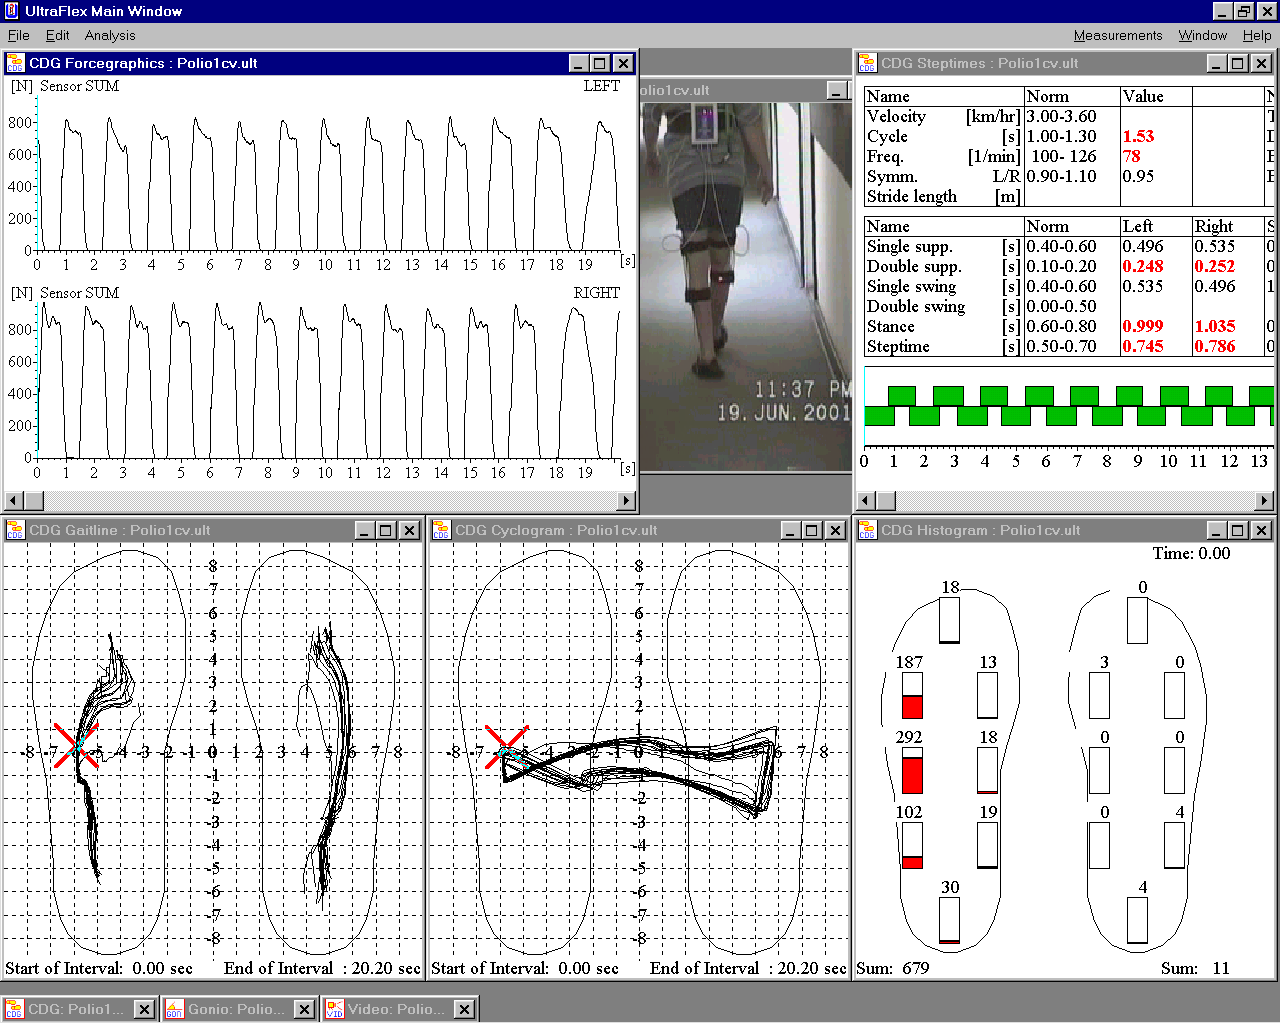
\includegraphics[scale=0.4]{./img/ultraflexdinografia.png}
 % matrixargseg.png: 296x162 pixel, 100dpi, 7.52x4.11 cm, bb=0 0 213 117
 %\caption{Estágio desenvolvimento de jogos ~\cite{fullerton2008game}}
\caption{\texit{Ultraflex Computer Dyno Graphy}}
%  \caption{Estágio desenvolvimento de jogos}
 \label{fig:dynography}
\end{figure}

\begin{figure}[!htbp]
 \centering
 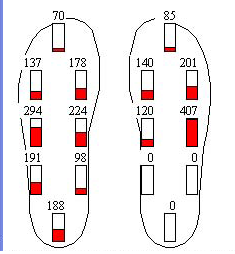
\includegraphics[scale=0.7]{./img/ultraflexposition.png}
 % matrixargseg.png: 296x162 pixel, 100dpi, 7.52x4.11 cm, bb=0 0 213 117
 %\caption{Estágio desenvolvimento de jogos ~\cite{fullerton2008game}}
\caption{Posição dos Sensores}
%  \caption{Estágio desenvolvimento de jogos}
 \label{fig:posicaosensores}
\end{figure}

A saída de cada um destes 16 sensores foi armazenada e gravada em 100 amostras por segundo, nesses registos estão inclusos dois sinais que refletem a soma da medição dos oito sensores para cada um dos pés sendo denominada de \ac{fvrs} do pé Esquerdo e Direito respectivamente ~\cite{gaitusingsensorsreview2012}, para esse trabalho foi utilizado o resultado desta soma para realizar a análise de movimento.

\subsection{Método}\label{section:metodo_parkinson_database}
Para a análise desses dados, foi utilizado um método de reconhecimento de faces bem estabelecido chamado de \textit{eigenfaces}~\cite{eigenfaces91}. Nós criamos o  método \textit{eigengaits} ~\cite{medeiros2013} para identificar características e padrões que pudesse classificar pessoas diagnosticadas com a doença de parkinson ante indivíduos sem o diagnóstico estabelecido.

A análise dos dados da \textit{Parkinson Disease Database} ~\cite{physionet}, incluiu 50 pacientes de Parkinson e 50 indivíduos que não possuíam desenvolvido a doença (segundo as informações fornecidas pela própria base de dados). Foram calculados, normalizados e escalonados em 80 \textit{frames} um total de 120 ciclos de marcha (Seção \ref{section:analise_marcha}) que foram usados para efetuar a técnica de aplicar a técnica \textit{eigengaits} ~\cite{medeiros2013} que é uma adaptação da Análise dos Componentes Principais que será explicada na Seção \ref{section:analise_marcha_pca}. 


\section{Estudo analítico de caso-controle}\label{section:estudo_caso_controle}
Esta etapa da pesquisa foi pautada pelo protocolo de pesquisa submetido à avaliação do Comitê de Ética da UFCG, somente após a aprovação deste (\textbf{CAAE: 14408213.9.1001.5182}) é que os dados foram coletados. 
Os resultados que se desejou alcançar com a pesquisa foi o descobrimento de mecanismos para a identificação e classificação de pessoas saudáveis ante os portadores de doença de parkinson. Durante a pesquisa também analisou-se o sensor de movimento MS-Kinnect ~\cite{kinnect2013} para avaliar a possibilidades de aquisição de dados de saúde baseada na Cinemática Linear do Movimento Humano.  

Através dos resultados obtidos pretendemos avaliar e classificar a normalidade e dificuldade na execução de movimentos como levantar um braço por exemplo.

A coleta de dados foi realizada nas seguintes instituições (Hospital Universitário UFAL, Fundação Pestalozzi - Maceió) sob a tutela da Profa. e Neurologista Dra. Cícera Pontes; e na Clínica de Fisioterapia do CESMAC sob a tutela do Prof. de Fisioterapia Jean Charles Santos, ambas realizadas em local reservado e de forma individual com a anuência do sujeito pesquisado através da assinatura do Termo de Consentimento.

\subsection{Amostra}
A técnica de amostragem utilizada para seleção, foi por conveniência onde foi composta por indivíduos 15 indivíduos diagnosticados com ~\ac{dp} e 12 indivíduos sem o diagnóstico como grupo de controle. 

\subsection{Recrutamento dos Sujeitos e Aquisição do Consentimento Livre e Esclarecido}
A forma de recrutamento deste protocolo será Circunscrita por intermédio de um profissional de saúde. O profissional deverá conhecer a história clínica do paciente e obterá a permissão do mesmo para que a equipe de pesquisa possa entrar em contato.
A equipe de pesquisa deverá explicitar os riscos e benefícios da participação da pesquisa buscando a espontaneidade da decisão e depois fornecer o Termo De Consentimento Livre E Esclarecido.

\subsection{Critérios de Inclusão}
Os indivíduos do grupo diagnosticados a \ac{dp} precisam estar no estágio 3 segundo a UPDRS ~\cite{updrs87}, sem distinção de sexo ou raça, que estejam dentro das facilidades da Clínica onde a coleta esteja sendo realizada e que aceitem participar do estudo.
Os indivíduos sem o diagnóstico da \ac{dp}, precisam informar que não possuem o diagnóstico da doença e aceitem a participar do estudo como grupo controle.

\subsection{Critérios de Exclusão}
Pessoas com sintomas motores e que tenham problemas em equilíbrio, questionamento de dores ao executar os procedimentos além daqueles que por qualquer motivo se negaram a participar do estudo.

\subsection{Materiais}
Para a presente pesquisa foi coletados movimentos de abdução e adução dos braços, que pudessem ser incorporados em um jogo eletrônico. Foi utilizado um jogo com o arcabouço de software de captura de dados desenvolvido por um aluno de Mestrado da Universidade Federal de Campina Grande ~\cite{antonio2013} juntamente com um aluno de iniciação científica do IFAL. Os dados foram coletados e depois processados e classificados com a abordagem apresentada nessa Proposta de Tese. 

Durante a execução desta coleta, houve uma preocupação com a integridade física dos participantes, muitos possuíam receio de quedas, logo os movimentos utilizados no jogo foram apenas de adução e abdução dos braços ~\cite{mcginnis2013biomechanics}, trazendo segurança aos participantes do grupo de indivíduos com \ac{dp}. 

\subsubsection{Infra-Estrutura}
A pesquisa será realizada na Clínica em que o paciente está em tratamento, onde são realizados tratamentos fisioterápicos ou consultas. O espaço físico forneceu condições favoráveis e adequadas para aplicação dos jogos. Para a realização da pesquisa foram utilizados:

\begin{itemize}
	\item Jogo (\textit{Catch the Spheres} rodando em notebook com Sistema Operacional Windows 7.0 e Unity 3d 3.0;
	\item Projetor (Epson Lcd Powerlite X14 3000l Hdmi) para projetar o jogo na parede e facilitar a visualização;
	\item Sensor de movimento Ms-Kinnect ~\cite{kinnect2013}.
\end{itemize}

\subsection{Métodos}
Essa pesquisa também fez uma análise de um sensor de movimento utilizados em jogos eletrônicos e avaliou a possibilidades de aquisição de dados de saúde baseada na Cinemática Angular do Movimento Humano ~\cite{hamill1999bases}.  Através dos resultados obtidos pretendemos avaliar e classificar a normalidade e dificuldade na execução de movimentos como abdução e adução dos braços.

A coleta de dados foi realizada no próprio espaço de tratamento do indivíduo em local reservado e de forma individual e permitindo sua participação por meio do Termo de Consentimento. Devido as restrições de tempo (1 minuto e 30 segundos) e a execução de um mesmo movimento por todos os participantes, foi solicitados que cada voluntário da pesquisa executassem os seguintes procedimentos:
\begin{enumerate}
	\item O voluntário se posiciona a uma distância de 2 metros do sensor de movimento, de modo a conseguir capturar toda a extensão superior do braço durante o movimento de abdução; 	
	\item O voluntário inicia o jogo \textit{Catch the Spheres} usando a mão esquerda conforme a interface da aplicação;
	\item O voluntário levanta 10 vezes o braço esquerdo e depois o braço direito o mais alto e mais rápido que consegue, de modo a permitir que fosse capturados a amplitude de movimento e a velocidade angular do mesmo. 
	\item O voluntário fecha a aplicação e esta realiza o armazenamento dos dados.
\end{enumerate}

\begin{figure}[!htbp]
 \centering
 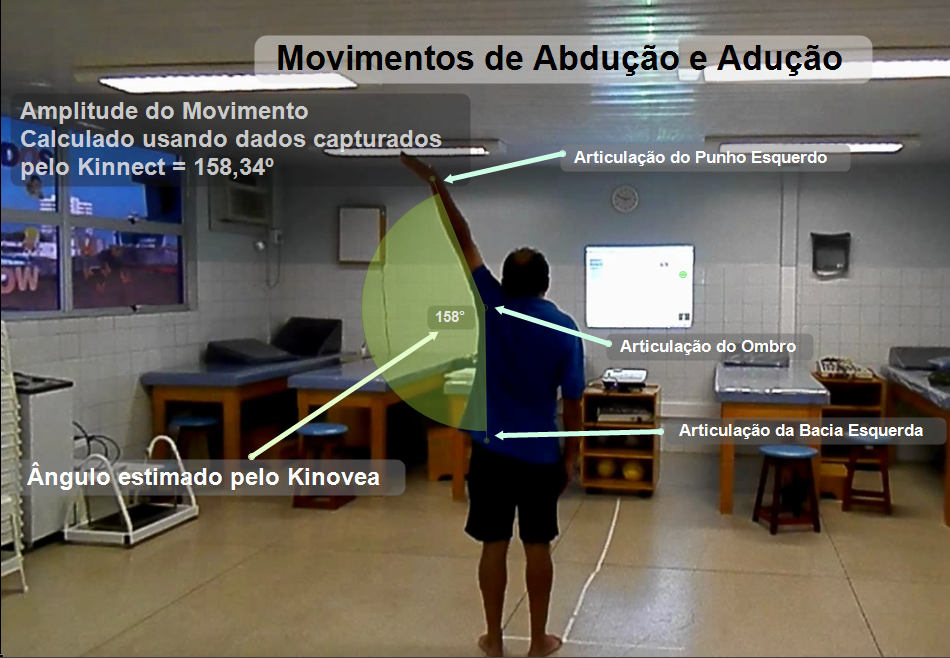
\includegraphics[scale=0.5]{./img/capturaducaokinnect.png}
 % matrixargseg.png: 296x162 pixel, 100dpi, 7.52x4.11 cm, bb=0 0 213 117
 %\caption{Estágio desenvolvimento de jogos ~\cite{fullerton2008game}}
\caption{Movimentos de Abdução e Adução}
%  \caption{Estágio desenvolvimento de jogos}
 \label{fig:movabducaomet}
\end{figure}

Durante a análise foram comparados os Ângulos Relativos do Tronco e do Levantamento de Braços dos Indivíduos. As grandezas cinemáticas coletadas nesses estudo foram:
\begin{enumerate}
	\item Do movimento de Abdução Figura \ref{fig:movabducaomet}, calculamos a amplitude máxima atingida por cada voluntário membros esquerdo e direito;
	\item Velocidade Angular de Abdução membros esquerdo e direito;
	\item Velocidade Angular de Adução membros esquerdo e direito.
\end{enumerate}

Esses dados biomecânicos foram coletados com o objetivo de identificar a bradicinesia nos indivíduos diagnosticados com a \ac{dp}ante os indivíduos sem o dianóstico da doença.
Pelo quantitativo da pesquisa ter sido de 27 indivíduos a abordagem de aprendizagem de máquina usando \ac{svm} ~\cite{vapnik95} foi utilizada juntamente com a técnica de validação-cruzada \textit{Leave One Out Cross-Validation} que será explicado com mais detalhes na \ref{chap:avaliacao}.


\subsection{Relação Risco e Benefício da Pesquisa}
Os riscos inerentes podem decorrer da exposição de dados dos sujeitos da pesquisa, o que pode acarretar danos morais e/ou psicológicos.

Assim, foram tomados todos os cuidados para que a identidade do sujeito da pesquisa não seja revelada, garantindo assim, privacidade e confidência das informações. Assim todos os dados do estudo foram manipulados apenas pelos principais pesquisadores, todos os dados serão armazenados sob criptografia, mitigando a possibilidade de vazamento da informação.

Caso ocorresse algum constrangimento por parte do sujeito da pesquisa, ao não conseguir realizar a pesquisa ou responder alguma pergunta devido ao comprometimento da doença. Os pesquisadores prestaram total assistência, orientando adequadamente os sujeito da pesquisa.

%Os presentes riscos fazem jus aos benefícios que a pesquisa venha a trazer com a possibilidade de monitoramento dos sintomas da \ac{dp}. A identificação dos sintomas motores e classificação desses dados através do computador podem permitir avanços para um melhor acompanhamento da evolução da doença além de possibilitar que os pacientes venham a ser monitorados de forma não invasiva através de um jogo eletrônico. Os pacientes deverão ter o seu estágio da \ac{dp} previamente diagnosticada por um médico para ser possível comparar os dados do monitoramento com a classificação obtida.



